\documentclass[12pt,a4paper]{article}
\usepackage{lipsum}
\usepackage[T1]{fontenc}
\usepackage[utf8]{inputenc}
\usepackage[noadjust]{cite}
\usepackage{authblk}
\usepackage[top=1in, bottom=1in, left=1in, right=1in]{geometry}
\usepackage{fancyhdr}
\usepackage{listings}
\usepackage{csquotes}
\usepackage{color}
\usepackage{setspace}
\usepackage{url}
\usepackage{graphicx}
\usepackage{float}
\usepackage{tabularx}
\usepackage{multirow}
\usepackage{adjustbox}
\usepackage{subfiles}
\usepackage{longtable}
\usepackage[utf8]{inputenc}
\usepackage[english]{babel}
\graphicspath{ {img/} }

\definecolor{gray}{rgb}{0.5,0.5,0.5}
\definecolor{lightgray}{rgb}{0.9,0.9,0.9}
\definecolor{editorGray}{rgb}{0.95, 0.95, 0.95}
\definecolor{editorMauve}{rgb}{0.58,0,0.82}
\definecolor{editorGreen}{rgb}{0, 0.5, 0} % #007C00 -> rgb(0, 124, 0)
\definecolor{editorBrown}{rgb}{.75, 0.375, 0} % #FF7F00 -> rgb(239, 169, 0)

\lstdefinelanguage{JavaScript}{
	morekeywords={typeof, new, true, false, catch, function, return, null, catch, switch, var, if, in, while, do, else, case, break},
	morecomment=[s]{/*}{*/},
	morecomment=[l]//,
	morestring=[b]",
	morestring=[b]'
}
\lstdefinelanguage{Bio}{
	morekeywords={A,C,G,T,a,c,g,t},
	alsoletter={<>\/()}
	morecomment=[s]{/*}{*/},
	morecomment=[l]//,
	morestring=[b]",
	morestring=[b]'
}
\lstdefinelanguage{HTML5}{
	language=html,
	sensitive=true, 
	alsoletter={<>=-},
	otherkeywords={
		% HTML tags
		<html>, <head>, <title>, </title>, <meta, />, </head>, <body>,
		<canvas, \/canvas>, <script>, </script>, </body>, </html>, <!, html>, <style>, </style>, ><
	},  
	ndkeywords={
		% General
		=,
		% HTML attributes
		charset=, id=, width=, height=,
		% CSS properties
		border:, transform:, -moz-transform:, transition-duration:, transition-property:, transition-timing-function:
	},  
	morecomment=[s]{<!--}{-->},
	tag=[s]
}

\lstset{%
	% Basic design
	backgroundcolor=\color{editorGray},
	basicstyle={\small\ttfamily},   
	frame=l,
	% Line numbers
	xleftmargin={0.75cm},
	numbers=left,
	stepnumber=1,
	firstnumber=1,
	numberfirstline=true,
	% Code design   
	keywordstyle=\color{blue}\bfseries,
	commentstyle=\color{editorGreen}\ttfamily,
	ndkeywordstyle=\color{editorBrown}\bfseries,
	stringstyle=\color{editorMauve},
	% Code
	language=HTML5,
	alsolanguage=JavaScript,
	alsodigit={.:;},
	tabsize=2,
	showtabs=false,
	showspaces=false,
	showstringspaces=false,
	extendedchars=true,
	breaklines=true,        
	% Support for German umlauts
	literate=%
	{Ö}{{\"O}}1
	{Ä}{{\"A}}1
	{Ü}{{\"U}}1
	{ß}{{\ss}}1
	{ü}{{\"u}}1
	{ä}{{\"a}}1
	{ö}{{\"o}}1
}

	
%
\pagestyle{fancy}
\fancyhf{}
\fancyhead[R]{\thepage}
%\lhead{APPLICATION OF COMPUTATIONAL METHODS TO STUDY THE SELECTION OF AUTHENTIC AND CRYPTIC SPLICE SITES}
%\fancyhead[L]{\fontsize{7}{12} \selectfont APPLICATION OF COMPUTATIONAL METHODS TO STUDY THE SELECTION OF AUTHENTIC AND CRYPTIC SPLICE SITES}
\setlength{\parindent}{0ex}
%
\begin{document}	
	%
	%title and author details
	
	\title{
	    {Application of Computational Methods to Study the Selection of Authentic and Cryptic Splice Sites}\\~\\~\\
	    {\large A Project}\\
	    {\large Presented to}\\
	    {\large The Faculty of the Department of Computer Science}\\
	    {\large San Jose State University}\\~\\~\\
	    {\large In Partial Fulfillment}\\
	    {\large of the Requirements for the Degree}\\
	    {\large Master of Science}\\~\\~\\
    }
    
    \author{By\\Tapomay Dey}
    \date{May 2017}
	\maketitle

	\thispagestyle{empty}
	\newpage
	\doublespacing
	\noindent

	\pagenumbering{gobble}
	\null\vfill
	\noindent
	\begin{center}
	\copyright 2017\\
	Tapomay Dey \\
	ALL RIGHTS RESERVED
	\end{center}
	\newpage	

	\thispagestyle{empty}
	\newpage
	\doublespacing
	\noindent

	\begin{center}
		\large ABSTRACT\\
	\end{center}
	Proteins are building blocks of the bodies of eukaryotes, and the process of synthesizing proteins from DNA is crucial for the good health of an organism \cite{khuri3}. However, some mutations in the DNA may disrupt the selection of 5' or 3' splice sites by a splicesome. An important research question is whether the disruptions have a stochastic relation to the position of nucleotides in vicinity of the known authentic and cryptic splice sites. This can be achieved by proving that the authentic and cryptic splice sites are intrinsically different. However, the behavior of the spliceosome is not accurately known. Hence, it is a logical step to model the behavior of the spliceosome using an algorithm that is suitable for modeling unknown functions. \par
	Genetic Algorithms have played an important role in heuristically optimizing NP-Hard search problems \cite{handbook}. An exhaustive search on the splice site data search space in order to determine the spliceosome function is an NP-Hard problem. Thus, spliceosome function is modelled as a search problem and a Genetic Algorithms based framework is created to prove the hypothesis. \par
	A Random Forest based classifier is proposed to be used as the scoring function. It reduces the rigidity of the comparison mechanism used to compare authentic and cryptic splice sites.
    	
    \thispagestyle{empty}
    \newpage
	\begin{center}
		\large ACKNOWLEDGEMENTS\\
	\end{center}
	I would like to thank my advisor, Dr. Sami Khuri, for teaching me many advanced topics in Computer Science and BioInformatics. His consistency in providing timely guidance and unique style of mentoring played a key role in the success of this project.\par
	I would like to thank Dr. Philip Heller and Dr. Thomas Austin for their invaluable inputs and guidance. \par
	I would also like to thank Dr. Sharmin Khan, Dr. Mark Stamp, Dr. Jon Pearce, and all my previous mentors.
	I am also grateful to my family and friends for supporting this venture of mine.

    \thispagestyle{empty}
	\newpage
	
	\tableofcontents
	
	\thispagestyle{empty}
	\newpage
	
	%tables
	\listoftables
	
	\thispagestyle{empty}
	\newpage
	
	%figures
	\listoffigures
	
	\thispagestyle{empty}
	\newpage
	%equations ?? nojoy
	
		
	\clearpage
    \pagenumbering{arabic}
    \doublespacing
	\section{\large Motivation}
    The eukaryotic genome consists of many genes. Transcription and translation are some of the important processes in the gene expression pathways. Transcription involves generation of messenger RNA (mRNA) from pre-messenger RNA (pre-mRNA). Both mRNA and pre-mRNA are sequences of nucleotides. The pre-mRNA is divided into nucleotide regions called Introns and Exons. An Exon-Intron boundary is called a 5’ splice site and an Intron-Exon boundary is called a 3’ splice spite. As per recent knowledge, the Introns are discarded and the Exons are stitched together to form the mRNA. \par
    The mRNA contains the coding sequence (CDS) that is translated into proteins. Proteins comprise of sequences made from various combinations of twenty possible amino acids. Each of the twenty amino acids can be mapped to multiple nucleotide triplets (codons) from the mRNA. One of the first publications of these mappings was by Crick in The Origin of the Genetic Code \cite{crick1}. The exact sequence of amino acids dictates the structural properties of the protein molecule. The structure and composition of a protein molecule influence the physical and chemical properties exhibited by the protein. These properties have been documented in the Wikipedia page on Amino Acids \cite{wiki-aminoacids}. \par
	\begin{figure}[h]
		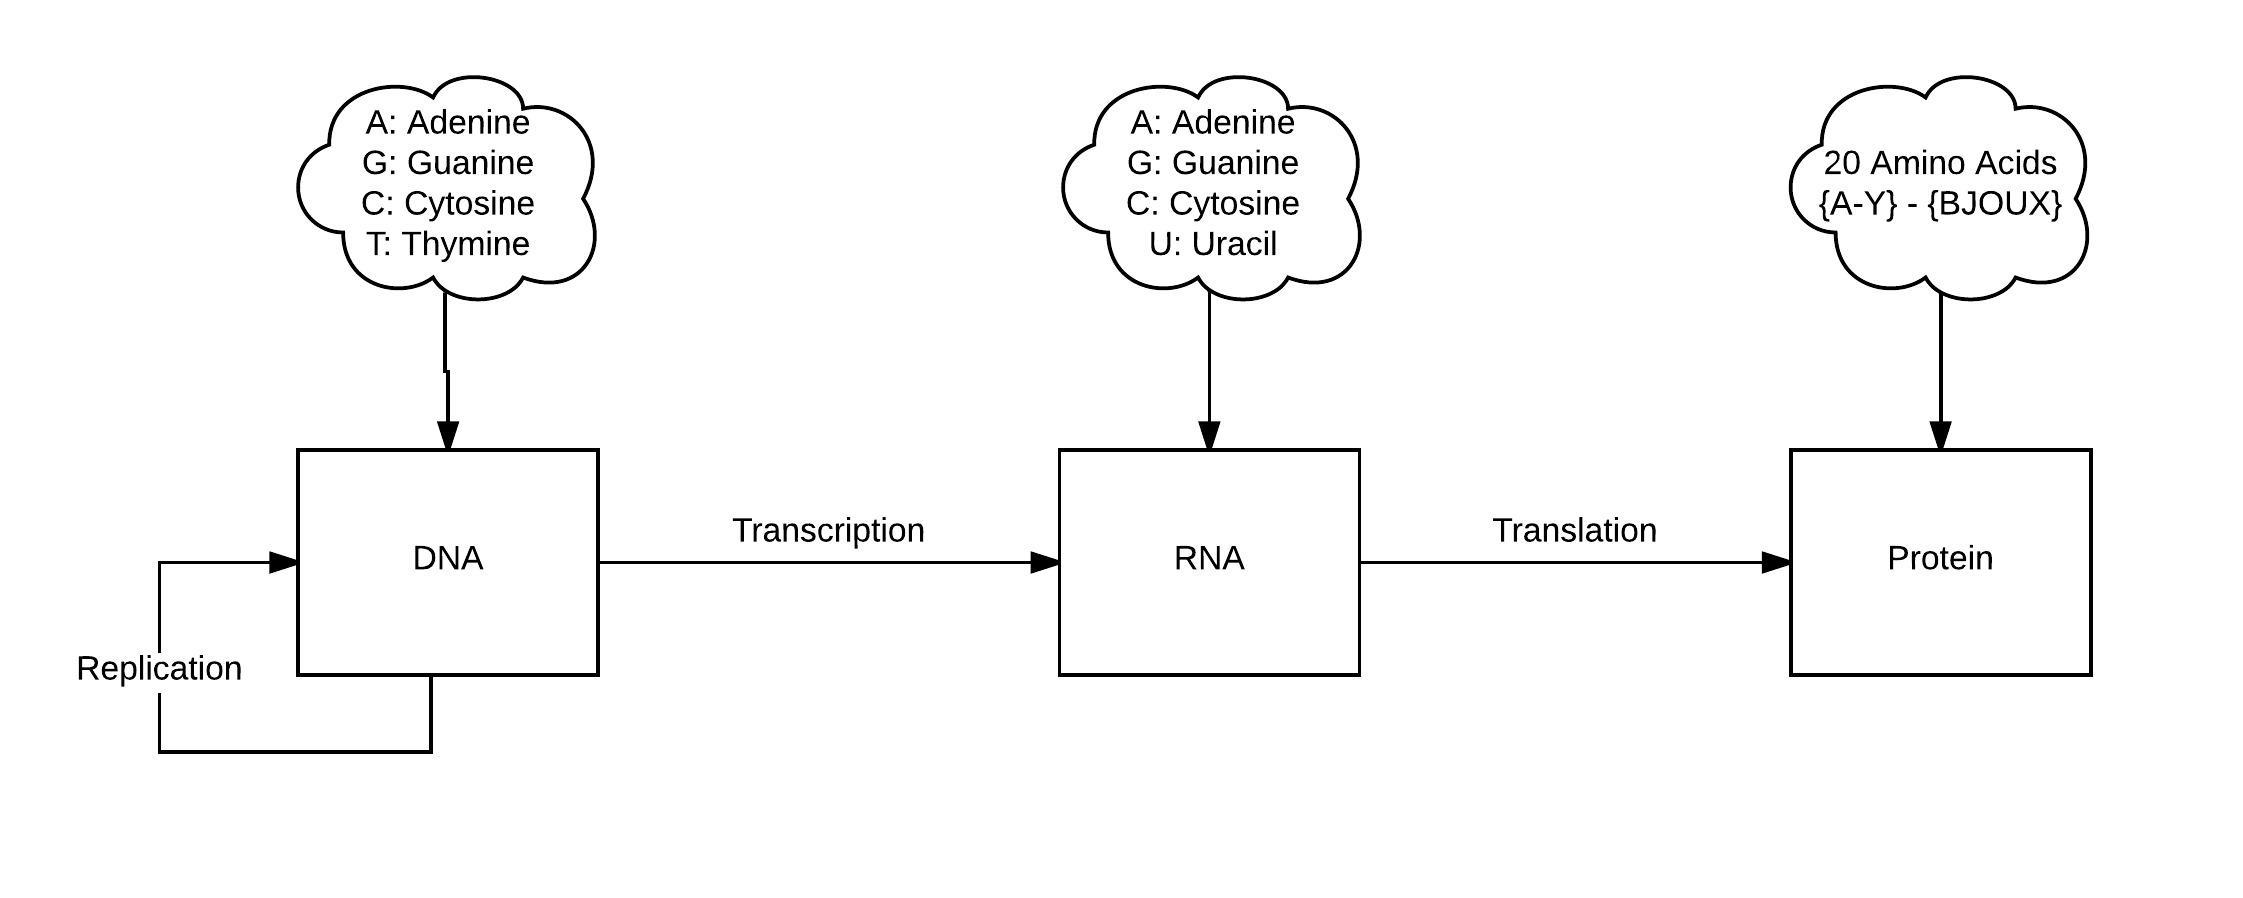
\includegraphics[width=\textwidth]{synthesis}
		\caption{Protein synthesis}
		\centering
	\end{figure}
	The proteins are responsible for various biological functions and traits of a eukaryotic organism. The splicing of pre-mRNA at 5’ and 3’ splice sites must be accurate in order to form the protein molecules that are required for satisfying the normally known functions of a healthy organism. \par
	Mutations in the DNA can lead to one of many possible disruptions in the selection of 5’ or 3’ splice sites. An obviously devastating disruption is a frame shift while extracting codons from the mRNA to form amino acid molecules. This may lead to a severely deficient expression of an important protein due to early detection of stop codons. In many cases, this leads to undesired consequences like fatal diseases. As per recent estimates, it is known that up to 50\% of disease-causing mutations disrupt splicing. \par
	The splice sites that are selected due to mis-splicing are called cryptic splice sites. However, there are multiple nucleotide subsequences in the pre-mRNA that contain candidate splice sites. Consequently, it is of crucial importance to understand the reasons behind the cryptic splice site selection by the spliceosome.
	

	\section{\large Problem Statement} \label{sec:problem}
	To study the selection of splice sites by the spliceosome, three data sets were built, consisting of authentic, cryptic, and neighboring 5’ splice sites. The data sets comprise of thousands of 9-mers: sequences that are 9 bases long. Authentic and cryptic splice sites are extracted from public datasets. The neighboring splice site 9-mers are extracted from 100 base-pairs downstream and 100 base-pairs upstream of each cryptic splice site. \par
	The primary goal is to build probabilistic models for each data set and quantitatively compare their similarities and differences. The primary hypothesis is that the authentic and cryptic splice sites are inherently different. The secondary hypothesis is that the neighboring splice sites are more dissimilar than both authentic and cryptic splice sites. This should help us understand the behavior of the spliceosome when it chooses cryptic splice sites and discards neighboring splice sites in case of mutations that disrupt the authentic splice site.
    
    \section{Data Specifications} \label{sec-dataspec}
    \subsection{5' Splice Sites}
    The 5’ splice sites are extracted based on the location of the invariant GT di-nucleotide. The authentic splice sites are extracted from the Homo Sapiens Splice Sites database (HS3D) \cite{hs3d-1,hs3d-2}. The cryptic splice sites and neighboring splice sites are extracted from the DBASS5 database \cite{dbass-0, dbass3}.
   	\begin{figure}[h]
   		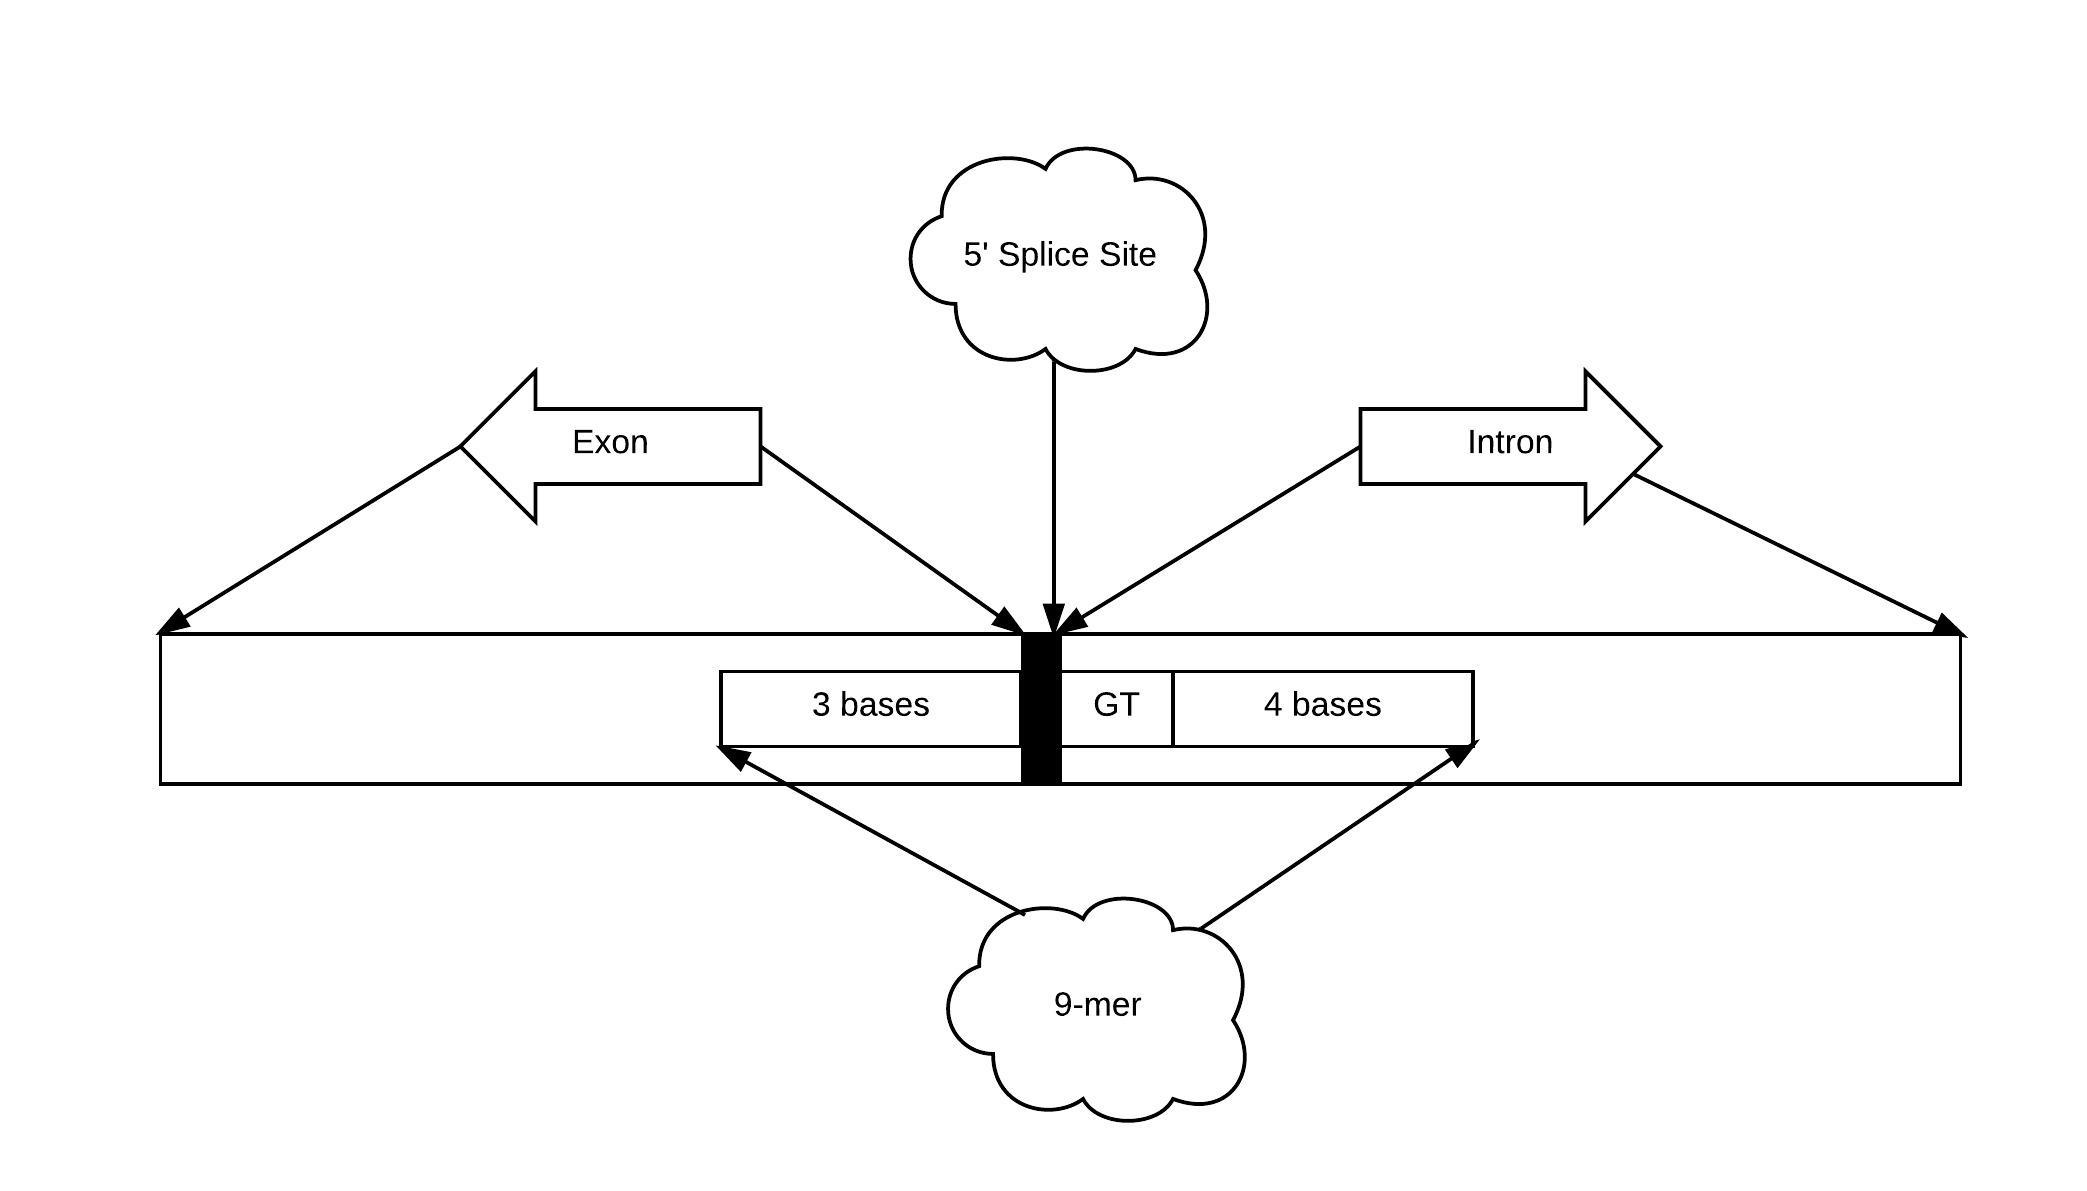
\includegraphics[width=\textwidth]{fiveprime}
   		\caption{5' Splice Site}
   		\centering
   	\end{figure}

	\subsection{Authentic 5' Splice Sites}
	HS3D offers the following files listed in figure-\ref{fig:hs3d_download} for download:
   	\begin{figure}[H]
   		\includegraphics[width=\textwidth]{"hs3d_download"}
   		\caption{HS3D downloads page}
   		\centering
   		\label{fig:hs3d_download}
   	\end{figure}
	\par Since 5’ splice sites occur at the Exon-Intron boundary, the file EI\_true.zip is relevant for Authentic 5’ splice sites. The data is provided as an ‘seq’ file with 140 nucleotides in each line. Manually observing all the sequences reveals that the 5’ consensus GT dinucleotide that marks the start of the Intron is at position 71-72 in each sequence. The desired 5’ splice site 9-mer comprises of the last 3 nucleotides from the Exon, the GT dinucleotide from the start of Intron and the 4 nucleotides following it. \par
	Following is a sample of 9-mers extracted from the dataset:
	
	\begin{table}[H]
	\caption{Input sequence lines from file EI\_true.seq}
	\begin{tabular}{ | p{\linewidth} |}
		\hline
		AB000381  ( 1,2,2): CTCCTCTTTGCCTTACTCCTAGCCATGGAGCTC \newline
		CCATTGGTGGCAGCCAGTGCCACCATGCGCGCTC\textbf{AGTGTAAGT}\newline
		ATCATTCCCTCTCACTGTCCTGGAGAGGACGAGAATTCCACCT\newline
		GGGGTGCTGGGGGTCACTGGG \\
		\hline
		AB000381  ( 2,3,3): AATGACTTCAACTGTCCCAACATTAGAGTATGT \newline
		CCGTATCATATTAGGCGCTGTATGACAATCTCCA\textbf{TTCGTAAGT}\newline
		ACCTCTTGGTCATTTGGACACATTGTAGATTAGTCCCCTACCT\newline
		GGGTAGTTTCTGGGGCCAGGG \\
		\hline
        AB002059  ( 3,1,1): TGACCAGGAACTGGCGGGTGGGCGCCCTGCAGA \newline
		GGCTGCTGCAGTTTGGGATCGTGGTCTATGTGGT\textbf{AGGGTAAGA}\newline
		GAGAAGAGCTTTTGGCCAGGCTGGAGGGGCAAGGGAAGAGGTG\newline
		GGGGGTGGGGCTTGGTCCTGC \\
		\hline
		AB002059  ( 4,2,2): TTCCGTCACTCAGATCAAGGAGCTTGGAAACCG \newline
		GCTGTGGGATGTGGCCGACTTCGTGAAGCCACCT\textbf{CAGGTGGGG}\newline
		GCCCTGATGTTGCTGACGGGGGCGCAAGTCCTTTCCCCACTGA\newline
		CAGCCTGAACACCCGCCATGC \\
		\hline
	\end{tabular}
	\end{table}
	
	
	\begin{table}[H]		
		\caption{9-mers extracted from the sequences in Table 1}
		\begin{tabular}{ | c |}
			\hline
			AGT\textbf{GT}AAGT \\
			\hline
			TTC\textbf{GT}AAGT \\
			\hline
			AGG\textbf{GT}AAGA \\
			\hline
			CAG\textbf{GT}GGGG \\
			\hline
		\end{tabular}
		\centering		
	\end{table}
	
	Total authentic 5’ splice site 9-mers extracted : \textbf{2796}
	
	\subsection{Cryptic 5' Splice Sites}
	
	The cryptic 5’ splice sites are collected from the DBASS5 database portal \cite{dbass-0, dbass3} by crawling all available splice site details page. The splice site details page contains the nucleotide sequence with the context of the mutation that alters the splicing location. The mutation is indicated in the sequence with a greater than symbol. \par
	For example: (G>A) means G is replaced by A \newline
	The cryptic splice sites are denoted by the slash symbol. \newline
	Consider the following nucleotide sequence extracted from the first record.\newline
	URL: http://www.dbass.org.uk/DBASS5/viewsplicesite.aspx?id=627 (last retrieved: 04/23/2017)

		
	\begin{tabular}{ | p{\linewidth} |}
		\hline
		CCAGCAACTT GGCTCTTTTT GGAGAGCGGC TGGGCCTGGT TGGCCACAGC CCCAGTTCTG CCAGCCTGAA CTTCCTCCAT GCCCTGGAGG TCATGTTCAA ATCCACCGTC CAGCTCATGT TCATGCCCAG GAGCCTGTCT CGCTGGACCA GCCCCAA\textbf{G/G} TGTGGAAGGA GCACTTTGAG GCCTGGGACT GCATCTTCCA GTAC\textbf{(G>A)}g tgaggccagg gacccgggca gtgctatggg gaagggacac catgggggcc caatttctcc ctctccacca cccagtgggg aatggaggcc acagggaggg gtcggggatt cctcaccttc ctgccaggga gattggtgcg aggctggggc tgggctgggc tgatccggag aatttgggat gagagcaggg agacttgggt gtcggggcag tctgggcagg aggaggacac tgaaggatgt ctcccagcac caaagtctga gggctgcctc ccgctccccg \\
		\hline
	\end{tabular}
	\newline
	\newline
	In the above nucleotide sequence:
	\begin{itemize}
		\item Capital nucleotide symbols indicate the trailing part of the Exon
		\item Small nucleotide symbols indicate the leading part of the Intron
		\item Mutation is marked as : (G>A)
		\item Cryptic splice site is marked as : “GCCCCAAG/G TGTGGAAGG”
	\end{itemize}
	The cryptic 5’ splice site 9-mer extracted from the above sequence is: AAGGTGTGG \par
	Total cryptic 5’ splice site 9-mers extracted : \textbf{539}

	\subsection{3' Splice Sites}
	The 3’ splice sites are extracted based on the location of the invariant AG dinucleotide and its preceeding $Y_n$ consensus where Y is a Pyridine. The authentic splice sites are extracted from the Homo Sapiens Splice Sites database (HS3D) \cite{hs3d-1,hs3d-2}. The cryptic splice sites and neighboring splice sites are extracted from the DBASS3 database \cite{dbass-0,dbass-1,dbass-2}.
   	\begin{figure}[H]
   		\includegraphics[width=\textwidth]{"threeprime"}
   		\caption{3' Splice Site}
   		\centering
   	\end{figure}

	\subsection{Authentic 3' Splice Sites}
	Since 3’ splice sites occur at the Intron-Exon boundary, the file IE\_true.zip is relevant for Authentic 3’ splice sites. This data is also provided as an ‘seq’ file with 140 nucleotides in each line. Manually observing all the sequences reveals that the 3’ consensus AG dinucleotide that marks the end of the Exon is at position 69-70 in each sequence. The desired 3’ splice site 13-mer comprises of the last 12 nucleotides from positions 59-70 at the end of the Exon, and one nucleotide from the start of the Intron. \par
	Following is a sample of 13-mers extracted from the dataset:

	\begin{table}[H]
		\caption{Input sequence lines from IE\_true.seq}
		\begin{tabular}{ | p{\linewidth} |}
			\hline
			AB000381(1,1,2): GGCCAGGGGCATAGAGCTGGCCAAGGAGCCATGGCTCAC\newline
			TAACGTGTTGTATGGGGCT\textbf{CCTTCCCTTCAGG}TCCAGGCTCCTGCGTGAAG\newline
			TGATGCTCCTCTTTGCCTTACTCCTAGCCATGGAGCTCCCATTGGTGGCA \\
			\hline
			AB000381(2,2,3): GAGTGAGCTGGTAATGGGTGGAAAAGGCGTAGTGGAGCA\newline
			GAAGCCTGAAGCCTGCTTT\textbf{CTCCCCTCTCAGG}GACTTACAGTTTGAGATGC\newline
			CATGACTGTGCGGTCATAAATGACTTCAACTGTCCCAACATTAGAGTATG \\
			\hline
			AB000381(3,3,4): TGTATGTGCCTCAATATTTACAAGCAGAAAATGTGAAAT\newline
			CAATTATTTTCATTGCTGC\textbf{TTCTTTTTTTAGG}CATAAATTCTCGTGAACTAC\newline
			TTGTTTATAAGAACTGTACAAACAACTGCACATTTGTATATGCAGCTGA \\
			\hline
			AB002059(4,1,2): GTAGGGCTCAGCTCCGCCCCTGTCACTACACGCTGGGGA\newline
			CACACCACACTGCCCGACT\textbf{TCTCCTCCCCAGG}TGGGCGCTCCTCGCCAAAAA\newline
			AGGCTACCAGGAGCGGGACCTGGAACCCCAGTTTTCCATCATCACCAAA \\
			\hline
			AB002059(5,2,3): AGGCTGCCGGCTTCCGGCCTTTCCAGTCAACACGAGCCC\newline
			AGCCAGGCCAACCTTGAGA\textbf{CTTGCCTCCTAGG}GAGAGAACGTGTTCTTCTTG\newline
			GTGACCAACTTCCTTGTGACGCCAGCCCAAGTTCAGGGCAGATGCCCAG \\
			\hline
		\end{tabular}
	\end{table}
	
	\begin{table}[H]	
		\caption{13-mers extracted from the sequences in Table 3}	
		\begin{tabular}{ | c |}
			\hline
			CCTTCCCTTC\textbf{AG}G \\
			\hline
			CTCCCCTCTC\textbf{AG}G \\
			\hline
			TTCTTTTTTT\textbf{AG}G \\
			\hline
			TCTCCTCCCC\textbf{AG}G \\
			\hline
			CTTGCCTCCT\textbf{AG}G \\
			\hline
		\end{tabular}
		\centering
	\end{table}

	Total authentic 3’ splice site 13-mers extracted : \textbf{2880}
	\subsection{Cryptic 3' Splice Sites}
	The cryptic 3’ splice sites are collected from the DBASS3 database portal \cite{dbass-0,dbass-1,dbass-2} by crawling all available splice site details page. The fields on the DBASS3 splice site details pages are similar to the ones on the DBASS5 pages. \par 
	The desired 13-mer comprises of : 
	\begin{itemize}
		\item 10 nucleotides before the ag dinucleotide from the Intron
		\item the ag dinucleotide at the splice site marker from the Intron
		\item one nucleotide after the splice site marker from the Exon
	\end{itemize}
	Consider the following nucleotide sequence extracted from a record at \\ URL: http://www.dbass.org.uk/DBASS3/viewsplicesite.aspx?id=52 (last retrieved: 04/23/2017)\par
	\vspace{5mm}	
	\begin{tabular}{ | p{\linewidth} |}
		\hline
		gtaagggccg ggggcatttt ttctttctta aaaaaatttt tttttaagag atgggttctt gctatgctgc ccaggctggt cttaaattcc tagtctcaaa tgatcctccc acctcagcct caagtgtgag ccacctttgg ggcatcccca atccaggtcc ctggaagctc ttgggggggc atatctggtg gggagaaagc aggggttggg gaggccgaag aaggtcaggc cctcagctgc cttcatca\textbf{g/ t}tcccaccct cca\textbf{g/c}cccc \textbf{(a>g)}\textbf{(c>g)} ctcctcctgc agACAAGCTG GTGTCTAGGA ACTACCCGGA CCTGTCCTTG GGAGACTACT CCCTGCTCTG GAAAGCCCAC AAGAAGCTCA CCCGCTCAGC CCTGCTGCTG GGCATCCGTG ACTCCATGGA GCCAGTGGTG GAGCAGCTGA CCCAGGAGTT CTGTGAGgta \\
		\hline
	\end{tabular}
	\\
	\\
	In the above nucleotide sequence:
	\begin{itemize}
	\item Capital nucleotide symbols indicate the leading part of the Exon
	\item Small nucleotide symbols indicate the trailing part of the Intron
	\item Mutations are marked as : (a>g) and (c>g)
	Cryptic splice sites are marked as : “cagctgc cttcatcag/ ttcccaccct ccag/cccc”
	\end{itemize}
	There are two cryptic 3’ splice site 9-mers extracted from the above sequence. They are: “tgccttcatcagt” and “cccaccctccagc” \par
	Total cryptic 3’ splice site 13-mers extracted : \textbf{306}

	\subsection{Neighboring 5' Splice Sites}
	The putative splice sites around the known cryptic splice sites are called neighboring splice sites. These are the putative splice sites that were not selected for splicing by the spliceosome in the event of a mutation. Using the nucleotide sequences extracted from the DBASS5 splice site details pages. The 100 base-pairs upstream and 100 base-pairs downstream of the splice site are parsed to look for the GT dinucleotide. All such occurrences are captured in the neighboring 5’ splice site dataset in the form of 9-mers with the GT dinucleotide as the 4th and 5th bases.\par
	
	Total neighboring 5’ splice site 9-mers extracted : \textbf{2213} \par
	
	There are many candidate algorithms for using the datasets specified in this section to solve the problem. The next section emphasizes the importance of analyzing its search space and proposes a suitable algorithm for solving the problem.
	
	\section{Algorithm Selection}
	For the 5’ and 3' splice sites, we can model the problem statement as a search problem. The spliceosome binds to a specific subset of the entire 9-mer search space. The cardinality of each position in the 9-mer is four (equivalent to A, C, G, and T). In 5' splice sites, the positions 4 and 5 are always occupied by the GT di-nucleotide. Hence, the size of the 5' splice site search space is $ 4^{7} = 16384 $. This search space comprises of the authentic, cryptic, and neighboring splice sites. An important goal is to study the statistical properties of the known samples from these three categories of splice sites and prove that they are inherently different. \par
	Evolutionary Algorithms (EAs) are applicable to problems that have no known classical optimization methods \cite{handbook}. If a traditional method is applicable to solve a problem, then EA should not be used since traditional methods are more efficient in such a case. Since we do not understand the choices of a spliceosome completely, EAs are suitable for this problem. The section-\ref{sec:modelling} describes a Genetic Algorithm based approach.\par
	Three primary forms of EA:
	\begin{itemize}
	\item Evolutionary Programming
	\item Genetic Algorithms
	\item Evolutionary Strategies
	\end{itemize}
	
	Some of the early significant contributors to EA \cite{handbook}:
	\begin{itemize}
	\item Friedberg (1958)
	\item Fraser (1957)
	\item Bremermann (1962)
	\item Box and Draper (1969): Evolutionary Operation
	\item Spendley (1962)
	\item Fogel (1966): Evolutionary Programming
	\item Holland (1967): Genetic Algorithms
	\item Rechenberg (1965): Evolutionary Strategies
	\end{itemize}
	
	Some of the initial conferences on EA:
	\begin{itemize}
	\item Schwefel and Manner (1991): Int'l workshop
	\item Belew and Booker (1991): ICGA'91
	\item Fogel and Atmar (1992): EP'92
	\item Manner and Manderick (1992): PPSN'92
	\end{itemize}
	
	\subsection{Background on Genetic Algorithms}
	Genetic Algorithms were first proposed and analyzed by John Holland (1975). Genetic Algorithms are a type of EA that deal with search and optimization based on a fitness function. It follows the philosophy of survival of the fittest. It uses the mechanisms of natural biological selection and genetics. \par
	Genetic algorithms follow a generic domain agnostic framework. Hence, it has the advantage of being applicable to many problems. Some of the features that initially separated GA from other evolutionary approaches are:
	\begin{itemize}	
	\item Bitstring representation
	\item Proportional selection
	\item Crossover
	\end{itemize}
	Although, the representation and selection methods have advanced significantly, there is still a large emphasis on the crossover operation. Crossover is known to give GAs a distinctive advantage over other methods \cite{handbook}. \par
	
	%\renewcommand{\labelitemi}{$\textbullet$}
	General Terminology: \\
	- Population: A collection of individuals of size m \\
	- Individual: A single string of size m that is part of the population \par
   	\begin{figure}[H]
   		\includegraphics[width=\textwidth]{"population"}
   		\caption{Population and Individuals}
   		\centering
   	\end{figure}
	
	Biological terminology: \\
	- Generation: equivalent to a population \\
	- Chromosome: equivalent to an individual \\
	- Gene: Each of the n positions in a chromosome is called a gene. It can be treated as a variable and can take values from a fixed set of alleles \\
	- Allele: A fixed set of values that can be taken by a gene \par

   	\begin{figure}[H]
   		\includegraphics[width=\textwidth]{"generation"}
   		\caption{Chromosome, Gene, and Alleles}
   		\centering
   	\end{figure}

	Figure 7 shows a generic algorithmic framework for domain agnostic genetic algorithms. The selection strategy, fitness operator, crossover operator, and recombination strategy are customizable according to a need. The framework makes no assumptions about the initial population or the operators.
	
	\begin{figure}[H]
		\includegraphics[width=\textwidth,height=\textheight]{"GA-block1"}
		\caption{An algorithmic framework for genetic algorithms}
		\centering
		\label{fig-framework}
	\end{figure}
	
	The two phases that can be used to introduce bias \cite{handbook}: 
	\begin{itemize}
	\item Selection strategy
	\item Recombination / replacement strategy
	\end{itemize}
	
	\subsection{SELECTION STRATEGIES} 
	Selection strategy is responsible for selecting individuals from a population for mating.
	\subsubsection{ROULETTE WHEEL}
	The total fitness value of all individuals in the parent population is computed. The probability of each individual is calculated as the ratio of its fitness to the total fitness. However, this strategy may lead to weak selection pressure. \par
	Selection pressure is governed by the differences in selection probabilities of individuals. If the differences are too small then the selection pressure is low.
	The workaround for low selection pressure is to scale the fitness probabilities with respect to the worst fitness. However, this leads to excessive selection pressure. The best individual may take over the entire population within a few iterations \cite{handbook}. \par
	
	\subsubsection{RANKED SELECTION}
	The workaround for excessive selection pressure is to use ranked selection. The parent population is sorted by fitness. Probability of selection is a linear function of the ranks sorted by fitness.
	
	\subsubsection{TOURNAMENT SELECTION}
	A small subset of the parent population is selected at random and the individual with best fitness is chosen for mating. This is repeated m times. The selection pressure can be controlled by adjusting the set size.
	
	\subsubsection{ELITIST STRATEGY}
	This is more of a strategy post selection. All but one of the child population after selection are chosen. The best individual from the parent population is added to the child population.
	
	\subsection{REPLACEMENT STRATEGIES} 
	A child population is generated from the parent population P(t) using selection, crossover, and mutation operations. A suitable replacement strategy is required to form the population for the next generation P(t+1) using candidate individuals from both the parent and child populations \cite{handbook}. 
	
	Some of the notable GA implementations that implement complex replacement strategies are:
	\begin{itemize}
	\item Whitleys GENITOR
	\item Syswerda’s steady-state GA
	\item Eshelman’s CHC
	\item Mühlenbein’s breeder GA
	\end{itemize}
	
	\subsubsection{REPLACEMENT STRATEGY ABSTRACTIONS}
	Let us assume:
	\begin{itemize}
	\item $\mu$: parent population
	\item $\lambda$: child population
	\end{itemize}
	
	\subsubsection{($\mu$ + $\lambda$) ES}
	The $\mu$ parents and $\lambda$ children are merged and the best $\mu$ individuals are chosen to form the new parent population.
	
	\subsubsection{($\mu$, $\lambda$) ES}
	The $\mu$ parents produce $\lambda$ offsprings such that $\lambda$ > $\mu$. The best $\mu$ offsprings out of the $\lambda$ offsprings are chosen to form the new parent population.
	
	\subsubsection{REPLACEMENT STRATEGY: OTHER VARIATIONS}
	Two other degrees of variation in a replacement strategy:
	\begin{itemize}
	\item Number of matings per iteration: \\
	Whether the GA produces one or two versus many ($\mu$) offsprings in each iteration; De Jong and Sarma (1993) claim that the main difference between variations in number of allowed matings is that a strategy with fewer matings leads to higher variance in performance.
	\item Whether the replacement strategy is biased or not: \\
	In case of an unbiased replacement strategy, if all the parents are replaced by the children, then we risk losing good individuals from the parent population for good. An advantage of this strategy is that the algorithm may wander out of a local minimum.
	\end{itemize}
	
	\subsubsection{MOST COMMON PRACTICAL REPLACEMENT STRATEGIES}
	\cite{goldberg}
	\begin{itemize}
	\item Delete All: \\
	All the child population replaces the entire current population
	\item Steady-state: \\
	Only n members of the current population are replaced by members from the child population; The quantity n and the strategy for removal are parametrized
	\item Steady-state-no-duplicates: \\
	Same as the Steady-state strategy except that the algorithm checks for duplicates while introducing chromosomes from the child population into the current population
	\end{itemize}

	\subsection{MUTATION}
	Mutation is the mechanism for producing variations by randomly replacing one allele with another. A commonly used rate of mutation is one over length of the string.

	\subsection{CROSSOVER}
	Crossover combines features from two highly fit individuals. The individuals maybe highly fit due to different reasons. However, we do not know which features account for the high fitness. Hence, the features are combined at random \cite{goldberg}.  \par
	Types of crossover \cite{goldberg}:
	\begin{itemize}
	\item One-point crossover
	\item Two-point crossover
	\item K-point crossover
	\item Uniform crossover
	\item Uniform order-based crossover
	\item Order-based crossover
	\item Partially matched crossover (PMX)
	\item Cycle crossover (CX)
	\end{itemize}

	For more details on each type of crossover, refer to how they are used with 9-mer data in section-\ref{sec:crossover}.

	\begin{figure}[H]
		\includegraphics[width=\textwidth,height=\textheight]{"GA-block2-algo"}
		\caption{Simple GA with one-point crossover, roulette wheel selection, and delete all strategy}
		\centering
	\end{figure}

	For more details on the crossover operators, refer how they are used with 9-mer data in the subsection-\ref{sec:crossover}. \par
	
	The selection strategies and crossover operators described in this section can be applied to the 5' and 3' splice site datasets, described in section-\ref{sec-dataspec}, using the algorithms specified in the next section.
	
	\section{MODELING THE PROBLEM STATEMENT USING GA} \label{sec:modelling}
	\subsection{DATA MODEL}
	Following is a logical mapping of the terminology shown in figure 6 to the splice site n-mer data:
	\begin{itemize}
		\item chromosome: an entire n-mer
		\item gene: each base in the n-mer
		\item allele: each base in the n-mer can take one of the following four nucleotides (A: Adenine, C: Cytosine, G: Guanine, T: Thymine)
	\end{itemize}
	
	\subsubsection{BASE\_MAP}
	In order to randomize allele generation or mutation, a random integer generator is used along with a mapping of alleles to integers. Each allele is mapped to an integer and the mapping is persisted as a global constant in the code. This mapping does not change across executions. \\
	- A: 1 \\
	- C: 2 \\
	- G: 3 \\
	- T: 4
	\subsubsection{9-mer}
	A chromosome for a 5’ splice site 9-mer is represented as a string of length 9 where each character belongs to the set {A, C, G, T} \par
	E.g.: AAAGTGTCC
	
	\subsubsection{13-mer}
	A chromosome for a 3’ splice site 13-mer is represented as a string of length 13 where each character belongs to the set {A, C, G, T} \par
	E.g.: AGATTCTCCCAGA
	
	\subsection{FITNESS FUNCTION: POSITION WEIGHT MATRIX} \label{sec-pwm}
	Position Weight Matrix (PWM) is a popular bioinformatic tool for predicting motifs in a sequence of nucleotides. It has also been found useful in many other applications involving sequence patterns and local multi-alignments. PWM has been successfully applied to representation of splice sites in nucleotide sequences \cite{pwm-2}. The PWM score of a motif is a useful measure of its strength \cite{pwm-1}. \par
	
	\begin{figure}[H]
		\label{fig:pwm}
		\includegraphics[width=\textwidth]{"pwm"}
		\caption{Position Weight Matrix: block diagram}
		\centering
	\end{figure}
	
	Figure-\ref{fig:pwm} shows the different phases involved in computation of a PWM from nucleotide sequences. \par
	\textbf{Algorithm: PWM} \\
	Given Inputs:
	\begin{itemize}
	\item Nucleotide sequences
	\item Nucleotide prior probabilities
	\end{itemize}
	
	\begin{lstlisting}[language=Python]
        symbolOddsMap = {A:0.28, C:0.22, G:0.22, T:0.28}
        freqMat = frequencyCounts(data, symbolSet, columnCount)
        laplacePWMMat = laplaceCountPWM(freqMat, symbolSet)
        logoddsMat = logodds(laplacePWMMat, symbolSet, symbolOddsMap)	
	\end{lstlisting}
	
	The logOdds matrix computed in step 4 is the PWM and can be used to score unknown sequences.\\
	Laplace pseudo count is used to handle zero values in step 3. \\
	The logodds matrix is the logarithm of a likelihood ratio. Hence, \\
	score > 0 $\Rightarrow$ positive sample \\
    score < 0 $\Rightarrow$ negative sample

	\subsection{ALGORITHMS: GA} \label{sec:algoGA}
	
	The high-level generic flow of the algorithm is as follows:
	\begin{enumerate}
		\item Build a probabilistic model of the input dataset
		\item Start with a random population
		\item Extrapolate a subset of the search space using the probabilistic model built in step 1
		\item Determine how much of the input dataset is covered by the subset of the search space extrapolated in step 3
	\end{enumerate}

	The input dataset comprises of the following types of splice sites:
	\begin{itemize}
		\item $A_5$: All known authentic 5’ splice sites
		\item $C_5$: All known cryptic 5’ splice sites
		\item $N_5$: All known neighboring 5' splice sites extracted as specified in section 3.7
		\item $A_3$: All known authentic 3’ splice sites
		\item $C_3$: All known cryptic 3’ splice sites		
	\end{itemize}
			
	For the sake of simplicity, let us consider only the 5' splice site datasets: $A_5$, $C_5$, and $N_5$.
	Let $S_5$ be the entire search space of 5' splice sites.
	$$|S_5| = 4^7 = 16384$$
	Without making any assumptions about the relation that exists between each dataset and $S_5$, we can state: 
	$$ A_5 \subset S_5 $$ 
	$$ C_5 \subset S_5 $$
	$$ N_5 \subset S_5 $$

	Now, we can define the following functions that map the entire search space to boolean values indicating membership to the known set of splice sites.
	$$ fcrypt_5:  S_5 \rightarrow Boolean; fcrypt_5(x)\textnormal{ = True  }\forall x \in C_5 $$
	$$ fauth_5: S_5 \rightarrow Boolean; fauth_5(x)\textnormal{ = True  }\forall x \in A_5 $$
	$$ fsplice_5: S_5 \rightarrow Boolean; fsplice_5(x)\textnormal{ = True  }\forall x \in \{A_5 U C_5\} $$
	
	Similarly, for 3’ splice sites, we can define the entire search space $S_3$ such that:
	$$ |S_3| = 4^{11} = 4194304 $$
	and we can define similar membership functions as follows:
	$$ fcrypt_3:  S_3 \rightarrow Boolean; fcrypt_3(x)\textnormal{ = True  }\forall x \in C_3 $$
	$$ fauth_3: S_3 \rightarrow Boolean; fauth_3(x)\textnormal{ = True  }\forall x \in A_3 $$
	$$ fsplice_3: S_3 \rightarrow Boolean; fsplice_3(x)\textnormal{ = True  }\forall x \in \{A_3 U C_3\} $$
	
	Now, we can redefine the problem statement defined in section-\ref{sec:problem} as follows:\\
	Can each membership function on chromosomes (fcrypt, fauth and fsplice) be defined in terms of simpler functions of the individual genes? \par
	
	We can use Genetic Algorithms to randomly extrapolate a subset of the search space $S_5$ with the help of a suitable fitness function. PWM is a highly sensible measure of statistical distribution of nucleotides in an n-mer. Hence, the PWM score of an n-mer is used as the fitness function for the Genetic Algorithm. The extrapolated subset of $S_5$ should have a high degree of similarity to the dataset used to train the PWM as compared to other datasets. \par
	
	\subsubsection{COMPUTING EXACT MATCH RATIO (EMR)}
	Let,
	\begin{itemize}
		\item $PWM\_A_5$ : PWM trained using $A_5$
		\item $PWM\_C_5$ : PWM trained using $C_5$
		\item $PWM\_N_5$ : PWM trained using $N_5$
		\item $EA_5$ : Subset of $S_5$ extrapolated using GA and $PWM\_A_5$
		\item $EC_5$ : Subset of $S_5$ extrapolated using GA and $PWM\_C_5$
		\item $EN_5$ : Subset of $S_5$ extrapolated using GA and $PWM\_N_5$
	\end{itemize}
	
	We compare the $EA_5$, $EC_5$, and $EN_5$ subsets based on their degree of similarity to the subsets $A_5$, $C_5$, and $N_5$. For the sake of simplicity, we compute degree of similarity using exact match ratio (EMR). \par
	Given two subsets S1 and S2, EMR can be defined as follows:
	\begin{equation}
		EMR(S1, S2) = |S2 \cap S1| / |S2|
		\label{eq-emr}
	\end{equation}
	
	For example, consider the following comparisons:\\
	$ EMR(EA_5, A_5) = |A_5 \cap EA_5| / |A_5| $ : Percentage of chromosomes in $A_5$ that are covered by $EA_5$ \\
	Similarly, we can define $ EMR(EA_5, C_5) = |C_5 \cap EA_5| / |C_5| $ \\
	In simpler terms, EMP(S1, S2) = ratio of individual n-mer strings in S2 covered by S1

	\subsubsection{COMPETING DATASETS} \label{sec:competing}
	Two datasets are competing if they are supposed to be intrinsically different as per the hypothesis.
	Thus,
	\begin{itemize}
	\item $A_5 \textnormal{ competes } C_5$
	\item $C_5 \textnormal{ competes } A_5$
	\item $N_5 \textnormal{ competes } A_5 \cup C_5$
	\end{itemize}

	\subsubsection{COMPARISON SCORES} \label{scores}
	Using the definition of EMR from equation-\ref{eq-emr}, we can define the score metrics that quantify the degree of similarity for comparing the datasets.\\
	Let us assume two datasets P and Q and their extrapolated sets EP and EQ (using GA with PWM). If P and Q are competing datasets (defined in section-\ref{sec:competing}, we can define the following comparison scores:
	\begin{itemize}
		\item PRESERVATION SCORE (PSCORE)
		\begin{equation}
			PSCORE(P) = EMR(EP, P)
			\label{eq-pscore}
		\end{equation}
		\begin{equation}
			PSCORE(Q) = EMR(EQ, Q)
		\end{equation}
		\item CONFUSION SCORE (CSCORE)
		\begin{equation}
			CSCORE(P) = 1 - EMR(EP, Q)
			\label{eq-cscore}
		\end{equation}
		\begin{equation}
			CSCORE(Q) = 1 - EMR(EQ, P)
		\end{equation}
	\end{itemize}
	If there exists a GA, that can give an EP and an EQ that maximize the scores PSCORE(P), PSCORE(Q), CSCORE(P), and CSCORE(Q), then we can conclude that P and Q are intrinsically different.
	
	\subsubsection{ENHANCED SCORES} \label{score-enhanced}
	The PSCORE and CSCORE measures are based on EMR, which looks for exact matches across the two participating datasets. The scores of the 3' splice sites are expected to be worse than the 5' splice sites because the 3' splice sites are longer and thus less probable to exactly match the known splice sites. Hence, the EMR based scores are too rigid for longer sequences. \par
	The coverage logic can be enhanced by considering local alignment scores instead of exact match. This should give us better coverage scores for 3' splice sites.
		
	\subsubsection{STEPS} \label{sec:steps}
	For 5' splice sites:\\
	Given datasets: $A_5, C_5,\textnormal{ and }N_5$
	\begin{enumerate}
		\item Compute $PWM\_A_5$, $PWM\_C_5$, and $PWM\_N_5$ from $A_5$, $C_5$, and $N_5$ respectively
		\item Initialize a random initial population P(1) of 9-mers with the GT di-nucleotide at positions 4 and 5
		\item Using $PWM\_A_5$ and a suitable GA parameters, extrapolate $EA_5$ from P(1)
		\item Using $PWM\_C_5$ and a suitable GA parameters, extrapolate $EC_5$ from P(1)
		\item Using $PWM\_N_5$ and a suitable GA parameters, extrapolate $EN_5$ from P(1)
		\item Compute $PSCORE(A_5)$ and $CSCORE(A_5)$ given that $A_5$ and $C_5$ are competing
		\item Compute $PSCORE(C_5)$ and $CSCORE(C_5)$ given that $C_5$ and $A_5$ are competing
		\item Compute $PSCORE(N_5)$ and $CSCORE(N_5)$ given that $N_5$ and $A_5 \cup C_5$ are competing
	\end{enumerate}
	
	The steps for 3' splice sites are same as above. The given datasets for 3' splice sites are $A_3, C_3,\textnormal{ and }N_3$.
	
	\subsubsection{DATASET LIMITATIONS}
	For the sake of simplicity, the experiments presented in this report are performed on limited datasets that do not include all known splice sites. The datasets are specified in detail in section 3.
	
	\subsection{ALGORITHMS: OPERATORS AND STRATEGIES}
	\subsubsection{SELECTION STRATEGIES}	
	\begin{enumerate}
	\item Roulette Wheel Selection: \par
	Example: \\
	\begin{table}[H]
		\centering
		\caption{Sample data: Roulette Wheel Selection}
		\begin{tabular}{ |c|c|c|c|c| }
		\hline
		Label & Chromosome & Fitness & Probability & Cumulative Probability \\
		\hline
		\hline
		C1 & 1101010 & 30 & $30/80=0.375$ & 0.375 \\
		\hline
		C2 & 1011001 & 15 & $15/80=0.1875$ & 0.5625 \\
		\hline
		C3 & 0100110 & 10 & $10/80=0.125$ & 0.6875 \\
		\hline
		C4 & 1000101 & 5 & $5/80=0.0625$ & 0.75 \\
		\hline
		C5 & 1111000 & 20 & $20/80=0.25$ & 1 \\
		\hline
		\end{tabular}
	\end{table}	
	
	\begin{figure}[h]
		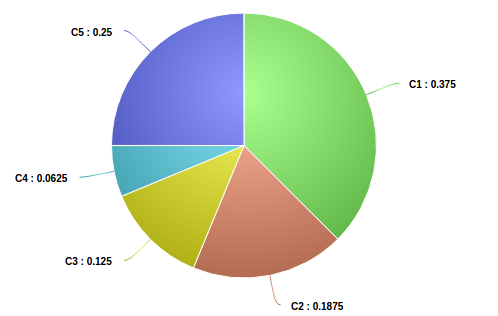
\includegraphics[width=\textwidth]{roulette-pie}
		\caption{Roulette wheel for chromosomes in Table 5}
		\centering
	\end{figure}

	
	\textbf{Algorithm:}\par
	A random number generator is used to generate a value $r \epsilon [0,1]$. The cumulative probabilities are used to select a chromosome. For example, if r = 0.7, then C4 is selected since $0.6875 < 0.7 < 0.75$
	\vspace{5mm}
	\begin{lstlisting}[language=Python]
    def rouletteWheel(population, fitnessFunction):
        fitnessArr = []
        for solution in population:
            fitness = fitnessFunction(solution) # compute fitness of each chromosome
            fitnessArr.append(fitness)
        
        minFitness = min(fitnessArr)
        fitnessArr = numpy.divide(fitnessArr, float(minFitness)) #scaling fitness values
        popFitness = float(sum(fitnessArr))   
        normFitnessArr = map(lambda x: x / popFitness, fitnessArr)  # normalize fitnessArr
        
        cumulative = 0
        normFitnessCumulativeArr = []
        for norm in normFitnessArr: # compute cumulative normalized fitness values
            cumulative = cumulative + norm
            normFitnessCumulativeArr.append(cumulative)
        
        ret = []
        for i in range(len(population)):
            spin = random.random()
            for j in range(1, len(normFitnessCumulativeArr)):
                if spin < normFitnessCumulativeArr[j]:
                    ret.append(population[j-1])
                    break
        return ret    
	\end{lstlisting}

	\item Ranked Selection: \par
	Example: \\
	Recomputing probabilities of the sample chromosomes from Table 5:
	\begin{table}[H]
		\centering
		\caption{Sample data: Ranked Selection}
		\begin{tabular}{ |c|c|c|c|c|c| }
			\hline
			Label & Chromosome & Fitness & Rank & Probability & Cumulative Probability \\
			\hline
			\hline
			C1 & 1101010 & 30 & 5 & $5/15=0.333$ & 0.333 \\
			\hline
			C2 & 1011001 & 15 & 3 & $3/15=0.2$ & 0.533 \\
			\hline
			C3 & 0100110 & 10 & 2 & $2/15=0.133$ & 0.666 \\
			\hline
			C4 & 1000101 & 5 & 1 & $1/15=0.067$ & 0.733 \\
			\hline
			C5 & 1111000 & 20 & 4 & $4/15=0.267$ & 1 \\
			\hline
		\end{tabular}
	\end{table}	
	
	\textbf{Algorithm:} \par
	We can re-use the roulette wheel selection algorithm after recomputing the fitness probabilities as a linear function of the ranks.
	\vspace{5mm}
	\begin{lstlisting}[language=Python]
    def ranked(population, fitnessFunction):
        fitnessTupleArr = []
        for solution in population:
            fitness = fitnessFunction(solution)
            fitnessTupleArr.append((solution, fitness))
        fitnessTupleArrSorted = sorted(fitnessTupleArr, key = lambda x:x[1]) # sort by fitness
    
        count = len(fitnessTupleArrSorted)
        popFitness = count * (count+1) / 2.0 # simulating rank order
    
        normFitnessTupArr = []
        idx = 1
        for tup in fitnessTupleArrSorted:
            rankProb = idx / popFitness
            normFitnessTupArr.append((tup[0], rankProb))
            idx += 1
    
        cumulative = 0
        normFitnessCumulativeArr = []
        for norm in normFitnessTupArr:
            cumulative = cumulative + norm[1]
            normFitnessCumulativeArr.append(cumulative)
    
        ret = []
        for i in range(len(population)):
            spin = random.random()
            for j in range(1, len(normFitnessCumulativeArr)):
                if spin < normFitnessCumulativeArr[j]:
                    ret.append(fitnessTupleArrSorted[j-1][0])
                    break
        return ret
	        
	\end{lstlisting}

	\item Tournament Selection: \par
	\textbf{Algorithm:} \par
	A fixed number (s) of random chromosomes are selected for a tournament. The chromosome with the highest fitness value among the s chromosomes is added to the mating pool. This process is repeated M times to select M chromosomes.
	\begin{lstlisting}[language=Python]
    def tournament(population, fitnessFunction, s=2):
        ret = []
        m = len(population)
        for idx in range(m):
            compete = random.sample(population, s)
            competeFitness = [fitnessFunction(individual) for individual in compete]
            winnerIdx = numpy.argmax(competeFitness)
            winner = compete[winnerIdx]
            ret.append(winner)
        return ret
	\end{lstlisting}

	\end{enumerate}

	\subsubsection{CROSSOVER OPERATORS} \label{sec:crossover}
	\begin{enumerate}

	\item One Point Crossover: \par
	
	Example:
	\begin{figure}[h]
		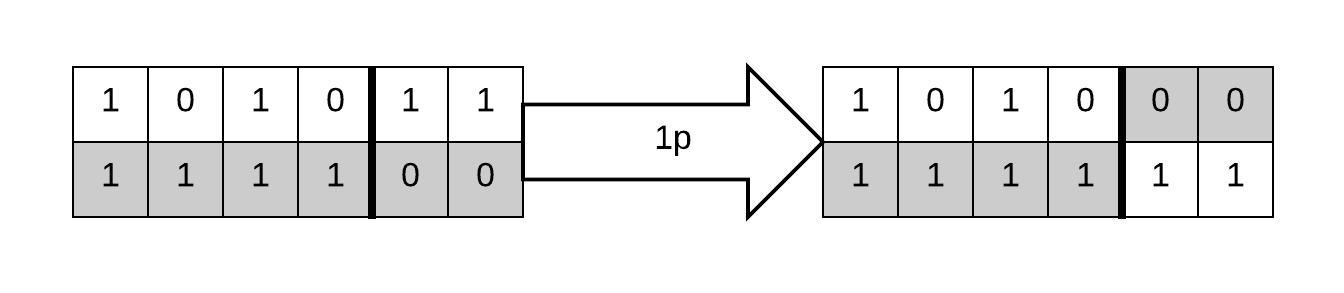
\includegraphics[width=\textwidth]{xover-1p}
		\caption{Example: One Point Crossover}
		\centering
	\end{figure}
	
	\textbf{Algorithm:} \par
	A crossover site is selected at random and all alleles on one side of the site are exchanged between the two parents.
	\begin{lstlisting}[language=Python]
    def uniform(parent1, parent2, swap_prob = 0.5):
        parentLen = len(parent1)
        child1 = parent1[:]
        child2 = parent2[:]
        for idx in range(parentLen):
            spin = random.random()
            if spin > 0.5: # perform allele swap at idx
                swap(child1, child2, idx)
        return (child1, child2)
	\end{lstlisting}

	\item Two Point Crossover: \par
	Example:
	\begin{figure}[h]
		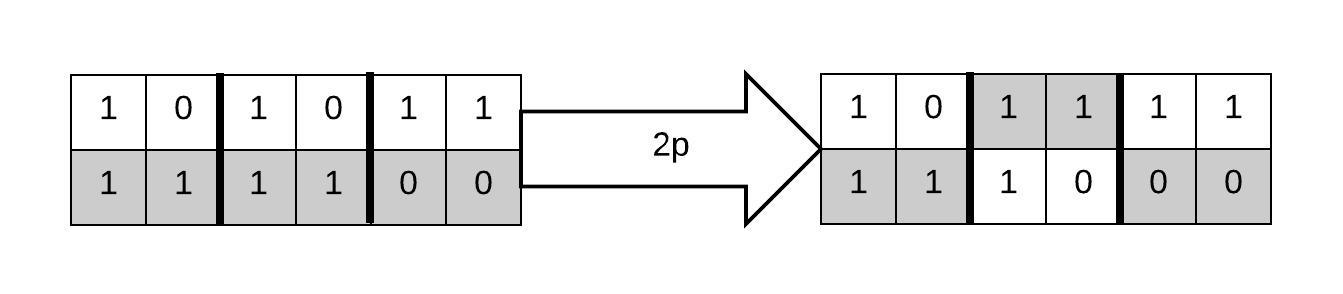
\includegraphics[width=\textwidth]{xover-2p}
		\caption{Example: Two Point Crossover}
		\centering
	\end{figure}
	
	\textbf{Algorithm:} \par
	Two crossover sites are selected at random and all alleles between the two sites are exchanged between the two parents.	
	
	\begin{lstlisting}[language=Python]
    def two_point(parent1, parent2):
        parentLen = len(parent1)
        site1 = pick_random_site(parentLen)
        site2 = pick_random_site(parentLen, negativeSites=[site1])    
        site1, site2 = sorted((site1, site2))
        p1_sub = parent1[site1:site2+1]
        p2_sub = parent2[site1:site2+1]
        child1 = parent1[0:site1] + p2_sub + parent1[site2+1:]
        child2 = parent2[0:site1] + p1_sub + parent2[site2+1:]
        return (child1, child2)
	\end{lstlisting}

	\item k-Point Crossover: \par
	The concept of 1-point or 2-point crossover can be extended to k points. The alleles between each odd crossover point and its immediately successive even crossover point are exchanged between the two parents.
	
	\item Uniform Crossover: \par
	Example:
	\begin{figure}[h]
		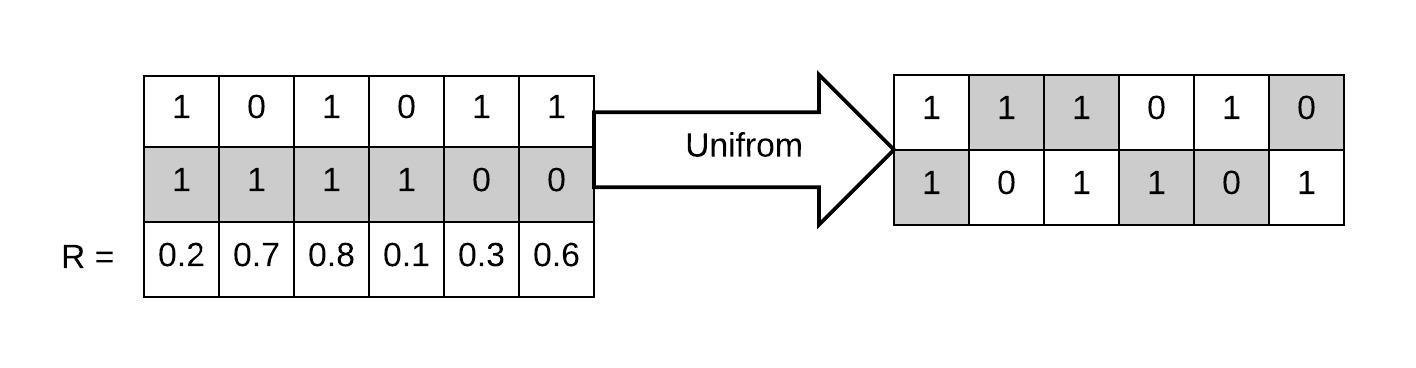
\includegraphics[width=\textwidth]{xover-uniform}
		\caption{Example: Uniform Crossover}
		\centering
	\end{figure}
	
	\textbf{Algorithm:} \par
	Each gene in the chromosome is considered for crossover with some swapping probability $p_{e}$. The alleles at the chosen gene locations ($R > p_{e}$) are swapped between the two parents.
	
	\begin{lstlisting}[language=Python]
    def uniform(parent1, parent2, swap_prob = 0.5):
        parentLen = len(parent1)
        child1 = parent1[:]
        child2 = parent2[:]
        for idx in range(parentLen):
            spin = random.random()
            if spin > 0.5: # perform allele swap at idx
                swap(child1, child2, idx)
        return (child1, child2)
	\end{lstlisting}

	\item Uniform Order-Based Crossover:
	Example:
	\begin{figure}[h]
		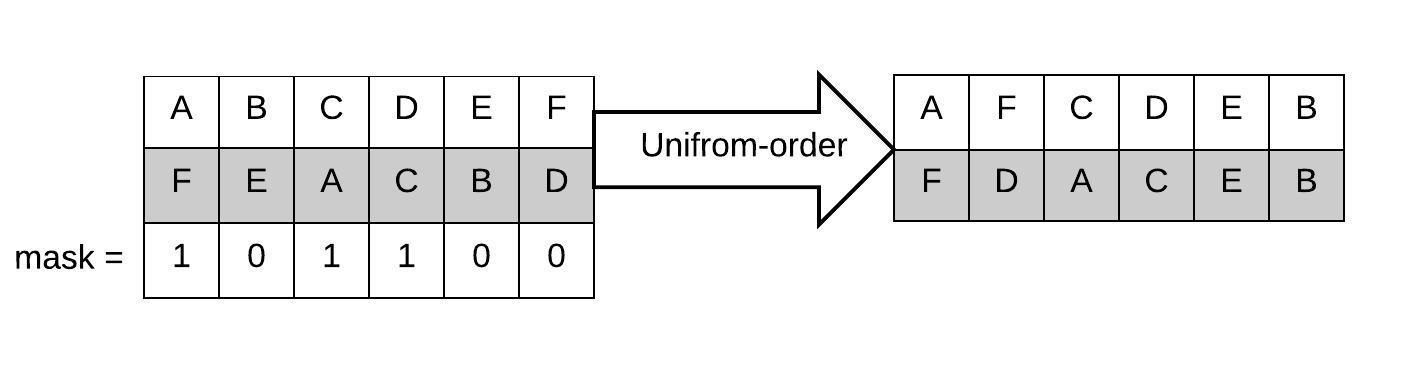
\includegraphics[width=\textwidth]{xover-uniformorder}
		\caption{Example: Uniform Order-Based Crossover}
		\centering
	\end{figure}
	
	\textbf{Algorithm:} \par
	A random binary template is used to guide the crossover. The alleles at indices in the parents corresponding to a 0 in the mask are reordered according to their order in the other chromosome.
	\begin{lstlisting}[language=Python]
    def uniform_orderbased(parent1, parent2):
        parentLen = len(parent1)
        child1 = parent1[:]
        child2 = parent2[:]
        maskStr = bin(random.getrandbits(parentLen)).replace('0b','')
        prefix = '0'*(parentLen - len(maskStr))
        maskStr = prefix + maskStr
        c1mask = [int(c) for c in maskStr]
        c2mask = [int(c) for c in maskStr]
    
        for neg in negativeSites:
            c1mask[neg] = 1
            c2mask[neg] = 1
    
        c1SwapSet = [child1[idx] for idx in range(parentLen) if c1mask[idx] == 0]
        c2SwapSet = [child2[idx] for idx in range(parentLen) if c2mask[idx] == 0]
        for idx in range(parentLen):
            allele = parent2[idx]
            if allele in c1SwapSet and 0 in c1mask:
                c1Idx = c1mask.index(0)
                child1[c1Idx] = allele
                c1mask[c1Idx] = 1
    
            allele = parent1[idx]
            if allele in c2SwapSet and 0 in c2mask:
                c2Idx = c2mask.index(0)
                child2[c2Idx] = allele
                c2mask[c2Idx] = 1
    
        return (child1, child2)

	\end{lstlisting}

	\if false
	\item Order-Based Crossover:
	\begin{lstlisting}[language=Python]
	\end{lstlisting}

	\item Partially Matched Crossover:
	\begin{lstlisting}[language=Python]
	\end{lstlisting}

	\item Uniform Crossover:
	\begin{lstlisting}[language=Python]
	\end{lstlisting}
	\fi
	
	\end{enumerate}
	
	All the operator and strategy algorithms specified in this section can be plugged into the parametrized GA framework defined in figure-\ref{fig-framework}. The next section presents the results of executing the GA framework for each combination of the operators and strategies. Since the result of one execution of a parametrized GA is stochastic, each instance of the parametrized GA is executed hundred times.
	
	\section{\large RESULTS} \label{sec-results}
		The algorithm defined in the steps section-\ref{sec:steps} is executed for each combination of the following parameters for GA:
		\begin{itemize}
			\item generation count: \{10, 100, 1000\} - number of generations
			\item generation size: \{10, 20\} - size of each generation
			\item selection strategy: \{roulette wheel, ranked, tournament\}
			\item crossover operator: \{one point, two point, uniform, uniform order based\}
		\end{itemize}
 
	\subsection{SCORING TABLES}
	The scoring tables are computed by executing each combination of the GA parameters 100 times.\par
	For the set of parameter values defined above, there are 3 X 2 X 3 X 4 = 72 parameter combinations. Each combination is executed 100 times in order to account for the stochastic nature of the results of each execution. \par
	Format of the scoring table:
	\begin{itemize}
		\item title of the table indicates the selection strategy and the crossover operator
		\item rows 1 - 3 indicate the dataset (AUTH, CSS, or NEIGHBOR), the score metric (PSCORE, CSCORE or FITNESS), and the GA paramters m (generation size) and gc (generation count)
		\item for a single set of parameter values for m and gc, there is a composite column comprising of two subcolumns f($\bar{x}$) and N. \\
		f($\bar{x}$) = unique value of the score metric \\
		N = frequency of the f($\bar{x}$) value across 100 execution
		\item the last row contains the mean of the score metric across all 100 execution
		\item row 5 to second last row contain the top eight f($\bar{x}$) values based on their frequency across the 100 executions
	\end{itemize}
	The scoring tables for the best performing parameter combination for each dataset with respect to the PSCORE, CSCORE, and FITNESS are listed in this section
	\subsection{SCORING TABLES: 5'}
	\subfile{CS298-draft1-results-best-5p}
	\subsection{SCORING TABLES: 3'}
	\subfile{CS298-draft1-results-best-3p}

	\subsection{SCORE SUMMARIES} 
	\subfile{CS298-draft1-summary-5p}
	\subfile{CS298-draft1-summary-3p}
	
	The summary tables \ref{score5} and \ref{score3} specify the best scores observed for each combination of dataset (Authentic splice sites, cryptic splice sites, and neighboring splice sites) and score metric (pscore, cscore, and fitness). \par
	We observe that the one point crossover, roulette wheel selection, and tournament selection dominate the scores for both 5' and 3' splice sites. \par
	Based on these results, it is highly interesting to filter the results and observe only the scores that contribute to the hypothesis the most. Such a point of interest is the cscores for cryptic splice sites that are specified in the next subsection.
	
	\subsubsection{POINT OF INTEREST: CSCORE FOR CRYPTIC SPLICE SITES}
	
	In this section, we aggregate the cscores for cryptic splice sites across all combinations of the GA parameters because we want to quantify the intrinsic difference or similarity between authentic and cryptic splice sites. Please note that by the definition of cscore in equation-\ref{eq-cscore}, since cryptic and authentic splice sites are competing datasets, it measures the dissimilarity between the datasets based on exact match ratio (equation-\ref{eq-emr}). A high cscore indicates high dissimilarity.
	
	\subfile{CS298-draft1-summary-css-cscores}
	
	In the tables \ref{tab-css-cscore3} and \ref{tab-css-cscore5}, we observe that the cscores are high across multiple selection and crossover operators. This proves that the cryptic splice sites are intrinsically different from authentic splice sites.
	
	Although, the results presented in this section are promising, the complexity of the GA for obtaining the results should not exceed an exhaustive search on the search space. The next section analyzes the time complexity of the GA for traversing the search space in order to construct the extrapolated 5' and 3' spice sites. 
	
	\section{ANALYSIS} \label{sec-analysis}
	\subsection{5' SPLICE SITE}
	The 5' splice sites are represented by a 9-mer with a fixed GT di-nucleotide in positions 4 and 5. Each position in the 9-mer has a cardinality of four corresponding to the four nucleotides - Adenine, Cytosine, Guanine, and Thymine. \\
	Search space size = $4^{9-2}$ = $4^7$ = \textbf{16384} \\
	The PWM-based genetic algorithm described in section-\ref{sec:modelling} extrapolates a subset of this search space. From the results described in table-\ref{score5} we can see that the algorithm converges decently close to the known splice site data in 1000 generations\\
	Given, \\
	Generation Count = 100 \\
	Generation size = 20 \\
	Number of 9-mers covered = $20 * 100 = 2000 $\\
	Search space coverage = $2000 / 16384 = 0.122$ \\
	Thus, by exploring only 12.2\% of the search space, we are able to approximately converge to a subset of the search space that is similar to known splice sites.

	\subsection{3' SPLICE SITE}
	The 3' splice sites are represented by a 13-mer with a fixed AG di-nucleotide in positions 11 and 12.
	Search space size = $4^{13-2}$ = $4^11$ = \textbf{4194304} \\
	Given, \\
	Generation Count = 100 \\
	Generation size = 20 \\
	Number of 9-mers covered = $20 * 100 = 2000 $\\
	Search space coverage = $2000 / 4194304 = 0.00047$ \\
	Thus, by exploring only 0.047\% of the search space, we are able to approximately converge to a subset of the search space that is similar to known splice sites.
	From the results described in section-\ref{score3} we can see that the algorithm converges decently close to the known splice site data in 100 generations\par

	\section{PHASE 2: CLASSIFICATION TEST USING EXTRAPOLATED SETS}
	
	In this section, we explore the performance of a classifier trained with the splice sites extrapolated by the GA. The known splice sites are tested with this classifier to measure the accuracy of the model. The main goal is to workaround the limitations of the exact match based scoring logic discussed in the section-\ref{score-enhanced}. The classifier based scoring should outperform the exact match based scores.
	
	\subfile{CS298-draft1-classification}

	\section{CONCLUSION}
	The results obtained in the section-\ref{sec-results} show that the mean fitness increases with generation count. This indicates that the the GA is successfully traversing the search space in a controlled fashion. Our time complexity analysis in section-\ref{sec-analysis} shows that the GA converges much faster than an exhaustive search space traversal. This becomes more evident in the analysis for 3' splice sites, which are longer n-mer splice site sequences. \par 
	The high similarity scores (pscore) in the summary tables \ref{score3} and \ref{score5} indicate a high similarity between the extrapolated set and the corresponding training splice site data. Similarly, the high dissimilarity scores (cscore) indicate a high dissimilarity between the extrapolated set and the corresponding competing (section-\ref{sec:competing}) splice site data. These observations provide us the evidence required to confirm the hypothesis that the competing splice sites are intrinsically dissimilar.\par
	The scores for the 3' splice sites are worse than the 5' splice sites. This is explained in section-\ref{score-enhanced}. The scores for the 3' splice sites can be improved by using local alignment-based algorithms for computing the scores because they are longer sequences than 5' splice sites. \par
	We also observed that the roulette wheel selection, tournament selection, and one point crossover give us most of the best scores across all combinations of GA parameters. \par
	Another interesting fact is that we get high scores in GA when we use PWM scores as fitness for the splice site datasets. The Position Weight Matrix is known to be a good probabilistic model for splice sites in nucleotide sequences \cite{pwm-2}. \par
	Some of the topics not covered here are schema theorem and analysis, representations and encoding techniques, and alternative random number generators. Schema analysis gives a more detailed understanding of the behavior of the GA. It is also used to compute a suitable crossover probability. Also, it has been shown that variations in the random number generator implementation have an impact on the performance of the GA. 
	
	%\section{APPENDIX}
	%\subfile{CS298-draft1-results-css-cscore-3p}
	
    \thispagestyle{empty}
    \newpage
	 
	\begin{thebibliography}{9}
		
		\bibitem{crick1}
		Crick, F. H. (1968).
		\textit{The origin of the genetic code. Journal of molecular biology, 38(3), 367-379.}
		Available [Online]: \url{https://profiles.nlm.nih.gov/ps/access/scbccb.pdf}
		Last retrieved: 04/26/2017
		
		\bibitem{wiki-aminoacids}
		Wikipedia
		\textit{Amino Acid}
		Available [Online]: \url{https://en.wikipedia.org/wiki/Amino_acid}
		Last retrieved: 04/26/2017

		\bibitem{hs3d-1}
		Pollastro, P., \& Rampone, S. (2003).
		\textit{ HS3D: homosapiens splice site data set. Nucleic Acids Research, (Annual Database).}
		Available [Online]: \url{ http://www.sci.unisannio.it/docenti/rampone/}
		Last retrieved: 04/26/2017

		\bibitem{hs3d-2}
		Pollastro, P., \& Rampone, S. (2002).
		\textit{ HS3D, a dataset of Homo Sapiens splice regions, and its extraction procedure from a major public database. International Journal of Modern Physics C, 13(08), 1105-1117.}
		Available [Online]: \url{https://www.researchgate.net/profile/Salvatore_Rampone/publication/2549884_HS3D_a_Dataset_of_Homo_Sapiens_Splice_Regions_and_its_Extraction_Procedure_from_a_Major_Public_Database/links/0912f510aade936928000000.pdf}
		Last retrieved: 04/26/2017

		\bibitem{dbass-0}
		\textit{DBASS: Database of Aberrant splice sites in human disease genes}
		Available [Online]: \url{http://www.dbass.org.uk/}
		Last retrieved: 04/26/2017

		\bibitem{dbass-1}
		Vorechovsky, I. (2006).
		\textit{Aberrant 3' splice sites in human disease genes: mutation pattern, nucleotide structure and comparison of computational tools that predict their utilization. Nucleic acids research, 34(16), 4630-4641.}
		Available [Online]: \url{https://academic.oup.com/nar/article/34/16/4630/3111901/Aberrant-3-splice-sites-in-human-disease-genes}
		Last retrieved: 04/26/2017

		\bibitem{dbass-2}
		Kralovicova, J., Christensen, M. B., \& Vorechovsky, I. (2005).
		\textit{ Biased exon/intron distribution of cryptic and de novo 3' splice sites. Nucleic acids research, 33(15), 4882-4898.}
		Available [Online]: \url{https://academic.oup.com/nar/article/33/15/4882/2401079/Biased-exon-intron-distribution-of-cryptic-and-de}
		Last retrieved: 04/26/2017

		\bibitem{dbass3}
		Buratti, E., Chivers, M., Kralovicova, J., Romano, M., Baralle, M., Krainer, A. R., \& Vorechovsky, I. (2007). 
		\textit{Aberrant 5' splice sites in human disease genes: mutation pattern, nucleotide structure and comparison of computational tools that predict their utilization. Nucleic acids research, 35(13), 4250-4263.}
		Available [Online]: \url{https://academic.oup.com/nar/article/35/13/4250/1203203/Aberrant-5-splice-sites-in-human-disease-genes}
		Last retrieved: 04/26/2017

		\bibitem{handbook}
		De Jong, K., Fogel, D., \& Schwefel, H. P. (1997). 
		\textit{Handbook of Evolutionary Computation. IOP Publishing Ltd and Oxford University Press.}
		Available [Online]: \url{http://citeseerx.ist.psu.edu/viewdoc/download?doi=10.1.1.375.6494&rep=rep1&type=pdf}
		Last retrieved: 04/26/2017

		\bibitem{goldberg}
		Sastry, K., Goldberg, D. E., \& Kendall, G. (2014).
		\textit{ Genetic algorithms. In Search methodologies (pp. 93-117). Springer US.}
		Available [Online]: \url{http://www.graham-kendall.com/papers/sgk2014.pdf}
		Last retrieved: 04/26/2017
		
		\bibitem{khuri1}
		Back, T., \& Khuri, S. (1994, June). 
		\textit{ An evolutionary heuristic for the maximum independent set problem. In Evolutionary Computation, 1994. IEEE World Congress on Computational Intelligence., Proceedings of the First IEEE Conference on (pp. 531-535). IEEE.}
		Available [Online]: \url{https://pdfs.semanticscholar.org/6881/7937ebf74d20c68e04ecc9b4aa04a4e8d8dc.pdf}
		Last retrieved: 04/26/2017

		\bibitem{khuri2}
		Khuri, S. (2012). 
		\textit{ Lecture Notes on Genetic Algorithms }

		\bibitem{khuri3}
		Khuri, S. (2017). 
		\textit{ Lecture Notes on BioInformatics }	    

		\bibitem{pwm-1}
		Xia, X. (2012).
		\textit{ Position weight matrix, gibbs sampler, and the associated significance tests in motif characterization and prediction. Scientifica, 2012.}
		Available [Online]: \url{http://downloads.hindawi.com/journals/scientifica/2012/917540.pdf} Last retrieved: 04/26/2017
		
		\bibitem{pwm-2}
		Claverie, J. M., \& Audic, S. (1996).
		\textit{The statistical significance of nucleotide position-weight matrix matches. Computer applications in the biosciences: CABIOS, 12(5), 431-439.}
		Available [Online]: \url{http://bioinformatics.oxfordjournals.org/content/12/5/431.full.pdf} Last retrieved: 04/26/2017
	    
		\bibitem{pangning}
		Pang-Ning, T., Steinbach, M., \& Kumar, V. (2006).  
		\textit{Introduction to data mining. In Library of congress (Vol. 74) }

		\bibitem{roc}
		Davis, J., \& Goadrich, M. (2006, June). 
		\textit{The relationship between Precision-Recall and ROC curves. In Proceedings of the 23rd international conference on Machine learning (pp. 233-240). ACM.}
		Available [Online]: \url{http://machinelearning.wustl.edu/mlpapers/paper_files/icml2006_DavisG06.pdf} Last retrieved: 04/26/2017

		\bibitem{rf1}
		Boulesteix, A. L., Janitza, S., Kruppa, J., \& König, I. R. (2012).
		\textit{Overview of random forest methodology and practical guidance with emphasis on computational biology and bioinformatics. Wiley Interdisciplinary Reviews: Data Mining and Knowledge Discovery, 2(6), 493-507. }
		Available [Online]: \url{https://epub.ub.uni-muenchen.de/13766/1/TR.pdf} Last retrieved: 04/26/2017

		\bibitem{rf2}
		Liaw, A., \& Wiener, M. (2002). 
		\textit{Classification and regression by randomForest. R news, 2(3), 18-22.}
		Available [Online]: \url{http://ai2-s2-pdfs.s3.amazonaws.com/6e63/3b41d93051375ef9135102d54fa097dc8cf8.pdf} Last retrieved: 04/26/2017
	    
	\end{thebibliography}
\end{document}
